\section{Methods}
\begin{figure*}
    \centering
    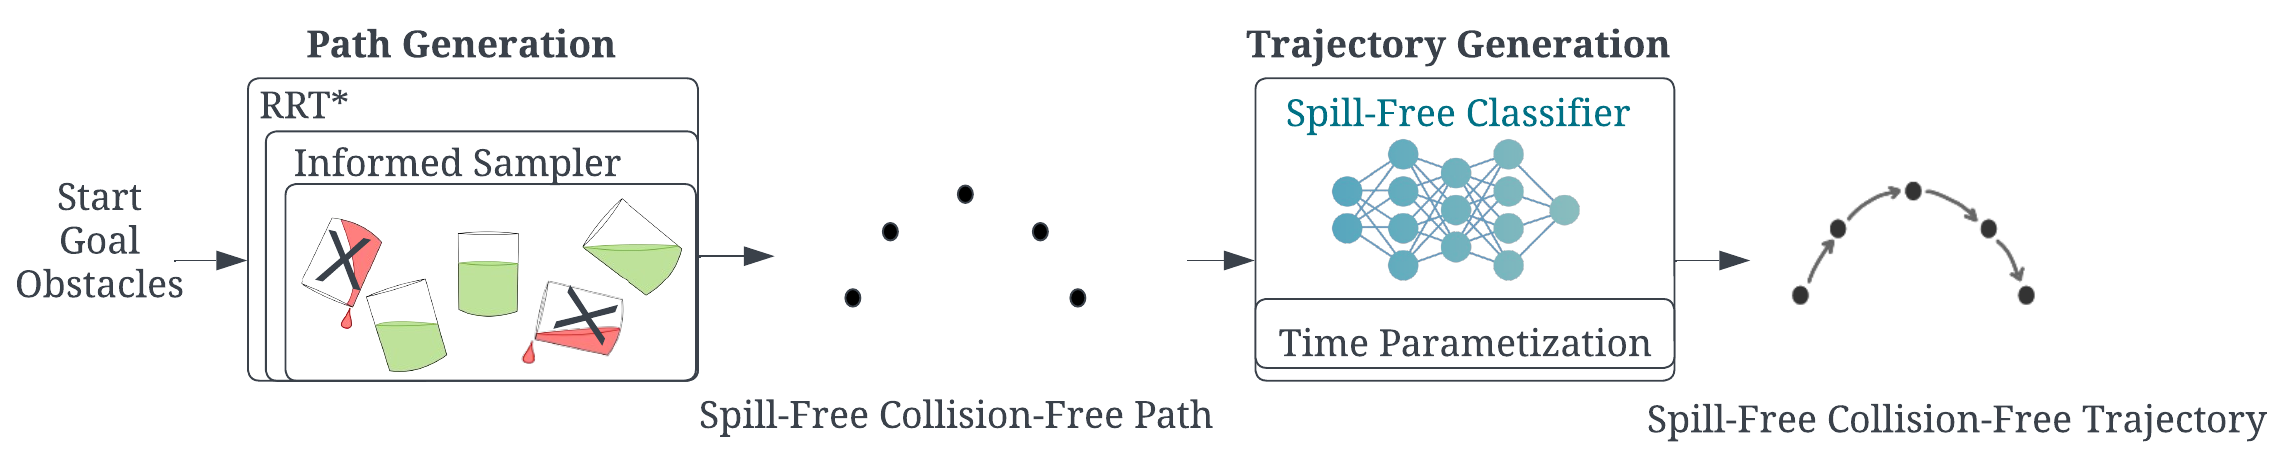
\includegraphics[width=\textwidth]{figs/sys_diagram_camera_ready_version.png}
    \caption{\textbf{System diagram}.
    The inputs are the start, goal, and obstacles, and the output is the trajectory. First, (i) a spill- and collision-free path is generated using RRT* and the informed sampler. The informed sampler utilizes the container properties to avoid sampling states such as an upside-down container. Then, (ii) a spill- and collision-free trajectory is generated using a time parameterization algorithm alongside the spill-free classifier model. The SFC model classifies trajectories as either spill-free or not and is utilized to set the jerk of the trajectory, ensuring the generation of a spill-free trajectory.}
    \label{fig:system_diagram}
    \vspace{-15pt}
\end{figure*}

This section introduces SFRRT*, a motion planner that generates spill- and collision-free trajectories (\cref{fig:system_diagram}).
SFRRT* accomplishes this through two key contributions: a) the informed sampler, mathematically formalized based on container geometry, to efficiently explore the space of spill-free robot states (\cref{subsec:informed-geometric-path-planner}), b) a transformer-based classifier that models the underlying nonlinear dynamics of liquid motion and classifies whether a planned trajectory is spill-free or not (\cref{method:timepar}).
% \input{2.5.problem_formulation} I don't have enough space for this
\subsection{Mathematical Formulation of the Spillage Scenario}
\label{subsec:cup_max_tilt_angle}
A challenge in spill-free trajectory generation is that the volume of the robot configuration space that contains spill-free trajectories is small and therefore inefficient to explore with random sampling alone \cite{zach}. This dictates the need for an informed approach to explore dynamically-valid robot states. However, developing a model for combined robot and object dynamics, specifically spillage dynamics, is computationally expensive, task-specific, and impractical for real-world control.
To address this, we need to mathematically formalize how container properties inform the construction of the \textit{spill-free space}. For example, for a given container that contains a greater volume of liquid, it cannot be tilted as much as when it contains less liquid. Additionally, in scenarios where containers have the same liquid volume, taller containers can be tilted more than shorter ones.


To sample spill-free configurations from the \textit{spill-free space}, we first calculate the maximum tilt angle that a container can withstand without spilling. Then, we sample states ensuring that their orientation remains within this range. Specifically, under quasi-static conditions, we consider the scenario that involves tilting a container to the point where it cannot retain all its content, i.e., to the angle $\theta_{max}$, such that any $\theta_{t} \leq \theta_{max}$ would be spill-free and any $\theta_t > \theta_{max}$ would cause spillage (\cref{fig:cup math}). Quasi-static conditions are assumed because they simplify analytical modeling without requiring expensive computational fluid dynamics calculations.


\begin{figure*}
\centering
\begin{subfigure}{0.32\textwidth}
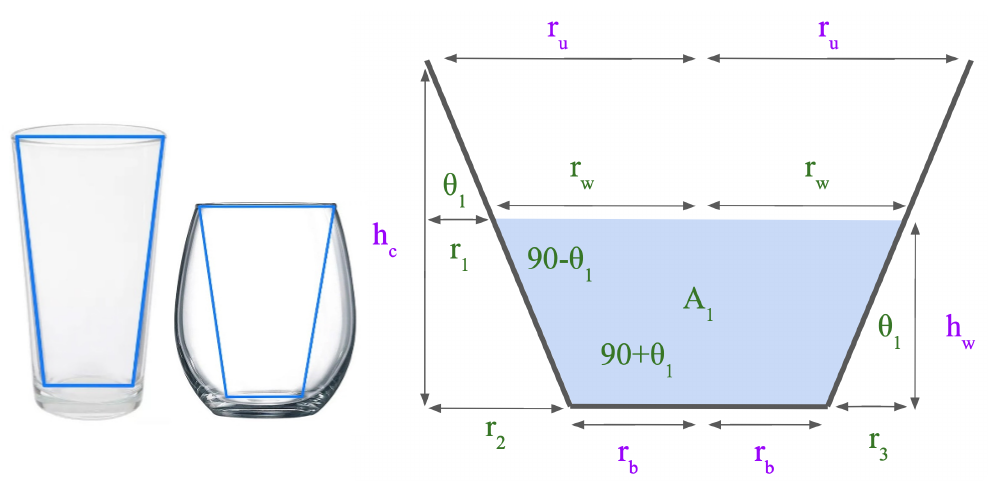
\includegraphics[width=\linewidth]{figs/cup_math_frustum_1.png}
\caption{Resting Position}
\label{fig:cup_math_rest}
\end{subfigure}
\hfill
\begin{subfigure}{0.30\textwidth}
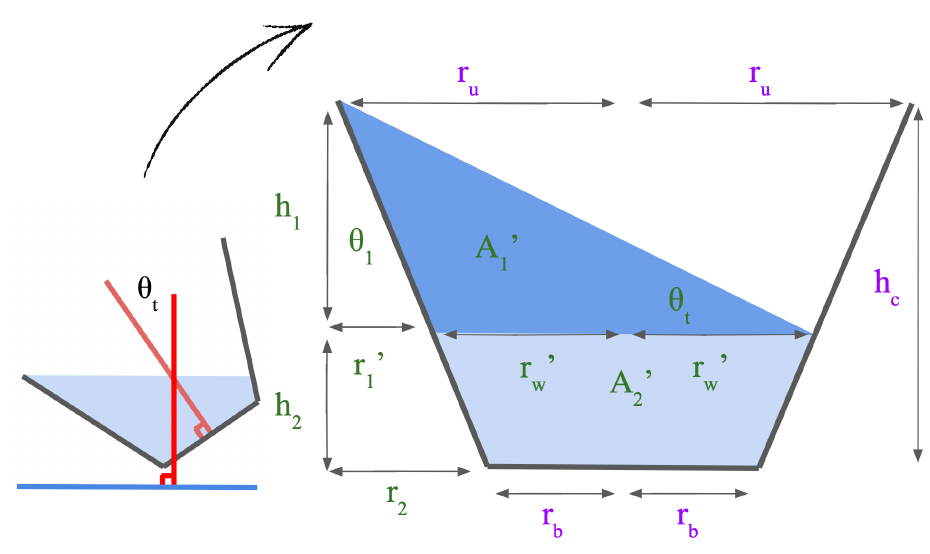
\includegraphics[width=\linewidth]{figs/tilt_case_2.png}
\caption{Case I}
\label{fig:cup_math_case_1}
\end{subfigure}
\hfill
\begin{subfigure}{0.30\textwidth}
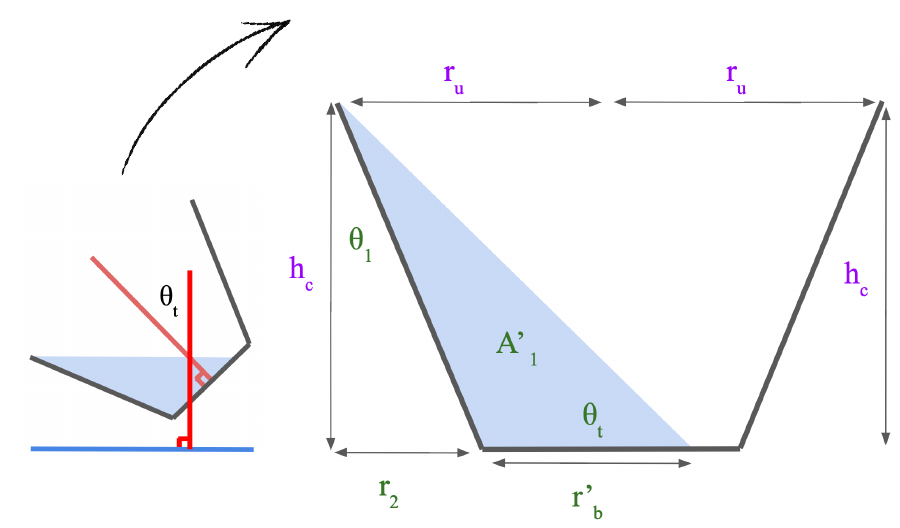
\includegraphics[width=\linewidth]{figs/tilt_case_3.png}
\caption{Case II}
\label{fig:cup_math_case_2}
\end{subfigure}
\caption{(a) depicts modeling containers as frustum of cones. Two cases occur when tilting the container as illustrated in (b) and (c). Case I is when the liquid forms both a trapezoid and a triangle shape. Case II shows when the liquid forms only a triangular shape. In both cases, $\theta_t$ represents the maximum tilt angle being calculated.
% \vspace{-15pt}
}
\label{fig:cup math}
\end{figure*}

To formalize the spillage scenario, we model the container as a frustum of a cone, which accurately represents most common container shapes and can provide an upper bound on the maximum tilt angle of containers with other shapes, such as round bottom flasks or curvy wine glasses (\cref{fig:cup_math_rest}).
% A frustum of a cone
Specifically, we simplify curved containers to the largest possible frustums of cones that can fit inside the original shape, leading to predicting spillage at a lesser tilt angle than the real container's capabilities. This guarantees a $\theta$ less than $\theta_{max}$, ensuring the generation of spill-free states. Lastly, we simplify the frustum of the cone representation from 3D to 2D, resulting in a trapezoid. This simplification also allows us to represent planar symmetric containers such as rectangular prisms and can be directly extended to 3D. 

To solve for the maximum tilt angle, we assume that the information we have from the container is the bottom circle radius $r_b$, the top circle radius $r_u$, the cup height $h_c$, and the water height $h_w$ (\cref{fig:cup_math_rest}). With this information, we can derive other relevant variables for calculating the maximum tilt angle. As shown in \cref{fig:cup math}, two spillage scenarios could occur: 
\begin{enumerate*}[label=(\roman*)]
\item one where the liquid forms a trapezoid and a triangle (\cref{fig:cup_math_case_1}), and
\item another where the liquid only forms a triangle (\cref{fig:cup_math_case_2}).
\end{enumerate*} This happens because static liquid stays parallel to the horizontal ground and depending on the liquid level, these cases can occur.

To calculate the maximum tilt angle, for both spillage cases, we leverage the key insight that the total amount of liquid remains constant before and after tilting the container. By equating the liquid area in the initial and tilted configurations, we derive an algebraic formula to compute the angle. The resulting equations, \cref{eq:caseI} for case I and \cref{eq:caseII} for case II, provide the respective maximum tilt angles.


Maximum tilt angle for case I:
\begin{equation}
% \begin{align}
\theta_{max} = tan^{-1} \left[\frac
{h_c(r_u-r_{w'})}
{(r_u-r_b)(r_u+r_{w'})}\right]
\label{eq:caseI}
% \end{align}
\end{equation}
where $r_{w'}= \frac{h_cr_ur_b - h_cr_2r_b + h_wr_2r_w + h_wr_2r_b}{h_cr_2 + h_cr_b}$.

Maximum tilt angle for case II:
\begin{equation}
\theta_{max} =tan^{-1} \left[ \frac
{h_c}
{r_u-r_b+(\frac{2h_w(r_w+r_b)}{h_c})}\right]
\label{eq:caseII}
\end{equation}
where $r_{w}= r_u-[(\frac{r_u-r_b}{h_c})(h_c-h_w)]$.

The next section explains how these equations are incorporated in the sampling-based path planner to inform the construction of a spill-free path.

\subsection{Informed Geometric Path Planning for Spill-Free Motions}
\label{subsec:informed-geometric-path-planner}
Having formalized the maximum tilt angle $\theta_{max}$, it is now used to guide the exploration of states that avoid spills, such as an upside-down container, or a container that is tilted beyond its capacity (i.e., $>$ $\theta_{max}$).
To achieve this, we implemented an informed sampler to sample robot configurations where the container orientation is less than the spill threshold $\theta_{max}$. Orientation refers to the container's Euler angles, and it is sampled such that the angle between the vertical axis and the axis about which the container is symmetric, is less than $\theta_{max}$. This informed sampler is then incorporated into a geometric RRT* path planner, to generate spill-free paths. RRT* is chosen due to its asymptotic optimality properties. By preferring transitions with minimal cost, RRT* generates smooth motion profiles that maintain orientation stability \cite{rrt*}. 
The next section describes how the path generated by RRT* is parameterized to ensure a spill-free trajectory.

\subsection{Time Parameterization To Create Spill-Free Trajectories}
\label{method:timepar}

While RRT* generates spill-free paths, to ensure the generation of a spill-free trajectory, we must carefully parameterize the path such that the velocity, acceleration, and jerk, do not cause spillage.
\begin{figure}
    \centering
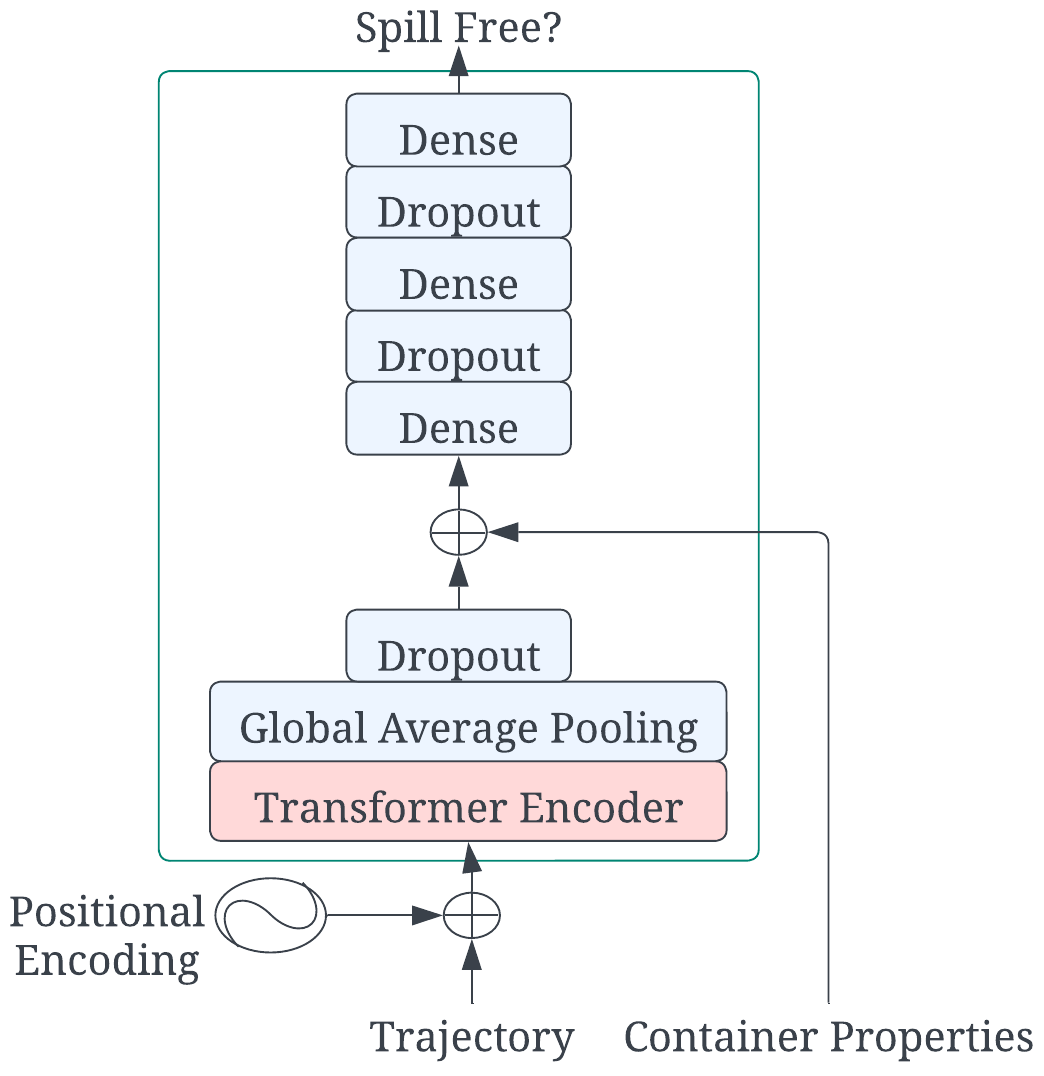
\includegraphics[width=0.8\columnwidth]{figs/model_camera_ready.png}\caption{\textbf{Spill-Free Classifier Model Architecture} The input is the trajectory and the container properties. The output is a boolean stating whether the trajectory is spill-free or not.
}
    \label{fig:models}
        % \vspace{-15pt}
\end{figure}
To do this, it is necessary to first model the risk of spillage with respect to the trajectory. To capture this relationship, we employed a transformer-based machine learning model trained to classify whether a container's trajectory is spill-free or not. This model is termed the \textit{Spill-Free Classifier} (SFC), and utilizes the transformer architecture, as depicted in \cref{fig:models}.

The input to SFC is the container trajectory and container properties, where the trajectory is the position and orientation over time and the properties represent the container's top and bottom radius, container height, and liquid fill level.
Furthermore, as shown in \cref{fig:models}, the trajectory is first passed through the transformer encoder layer. Then, the container properties are concatenated with it. The SFC model employs the transformer architecture because its input is sequence data (the trajectory) and transformers have become the leading architecture for handling sequential data due to their efficient parallel training capabilities and long context window \cite{huggingfacetransformers}. 

Lastly, to train the SFC model, we utilized a motion capture system to collect container trajectories (comprised of position and orientation over time) performed by individuals across different container types and liquid volumes (\cref{fig:Training set}). We collected a total of 700 trajectories, including 655 human-performed trajectories and 45 trajectories from the Panda robot. These trajectories encompassed a variety of paths from holding cups upside down and following zig-zag patterns to transporting cups in straight or typical paths between two points.
\begin{algorithm} \footnotesize
\caption{Spill Free Time Parametization (SFTP)} \label{alg:sftp}
\begin{algorithmic}[1]
\STATE {\bfseries Input:} Waypoints $\mathcal{W}$, Max Jerk $J_{max}$, Max Acceleration $A_{max}$, Max Velocity $V_{max}$, Jerk Decrease Factor $rate$, Max Iterations $N$,
\STATE {\bfseries Output:} Trajectory $\mathcal{T}$
\STATE $P_{s}, P_{f} \gets W[0]$, $W[length(W)-1]$
\STATE $V_{s}, V_{f}, A_{s}, A_{f} \gets 0$
\FOR{$ i = 1 ... N$} \label{sftp:loop}
    \STATE $\mathcal{T} \gets$ Ruckig($\mathcal{W}, J, V, A, P$)
    \STATE $\mathcal{T}_{fk} \gets ForwardKinematics(P)$ \label{sftp:fk}
    \STATE $spillFree \gets$ SpillFreeClassifier($\mathcal{T}_{fk}$) \label{sftp:sfc}
    \IF{$spillFree$}
        \RETURN $\mathcal{T}$ \label{sftp:stop}   
    \ELSE
    \STATE $J_{max} \gets \frac{J_{max}}{rate}$ \label{sftp:jerk_reduce}
    \ENDIF
\ENDFOR
\end{algorithmic}
\end{algorithm}


Having modeled the relationship between the container trajectory and spillage risk, we leverage SFC to generate spill-free trajectories. We introduce the \textit{Spill-Free Time Parameterization} (SFTP), which guarantees the creation of spill-free trajectories by utilizing a time-parameterization algorithm alongside the SFC model.
The key idea is to find the maximum jerk that does not cause spillage. To achieve this, SFTP works by iteratively (line \ref{sftp:loop}, \cref{alg:sftp}) reducing the maximum jerk of the trajectory (line \ref{sftp:jerk_reduce}, \cref{alg:sftp}), querying SFC after each iteration (line \ref{sftp:sfc}, \cref{alg:sftp}) until SFC predicts the resulting trajectory is spill-free. Jerk constraints are especially critical in preventing sudden changes in acceleration that could cause spillage. SFTP only modifies the jerk parameter since it directly affects acceleration and velocity. Lastly,  for time parameterization the Ruckig algorithm \cite{ruckig} is used since it can enforce constraints on higher-order derivatives including jerk, acceleration, and velocity.

In summary, to generate a spill-free collision-free trajectory (\cref{fig:system_diagram}), first, the container shape and fill level are leveraged to inform the generation of a path using RRT*. The spill-free classifier (SFC) model is then used alongside the Ruckig time-parameterization algorithm to ensure the generation of a spill-free trajectory. We refer to this combined process of generating the path and the trajectory, the \textit{spill-free RRT*} (SFRRT*) algorithm. 
